\section{Elementary Maths}
Should be fairly easy, this section is just so that everyone is one the same page and use the same notation for the rest of the course.
I will go fast as I assume you have already seen this before.
\subsection{Mathematical Objects \& Notations}
\subparagraph{Sets}
\begin{definition}[Sets]
    Unordered list of elements.
\end{definition}
\begin{notation}[Sets]
    $a \in A$, $\{ a, b, c \dots \}$, $\{ e \mid condition \}$, $\emptyset$
\end{notation}
\begin{remark}[Russell Paradox]
    \textit{(digression)}\\
    Need to be careful when defining set: some definitions are pathological.
    
    e.g.: Take $Y = \{x \mid x \not\in x\}$:
    $Y \in Y \iff Y \not\in Y$
\end{remark}

\subparagraph{Types of numbers}
\begin{definition}[Booleans]
    The set of boolean numbers $\B$ is $\{0,1\}$ or sometimes denoted $\{False, True\}$.\\
\end{definition}
\begin{definition}[Naturals]
    The set of natural numbers $\N$ is $\{0,1,2,3,\dots\}$.\\
    N.B.: some countries do not count $0$ as a natural number; but we are in France, so in this course, we will.\\
    N.B.(bis): If we need the naturals without zero, we will use $\N^*$.
\end{definition}
\begin{definition}[Integers]
    The set of integral numbers $\Z$ is $\{0,1,-1,2,-2,3,-3,\dots\}$.\\
    N.B.: If we need only the negative part of the integers, we will use $\Z^-$.
\end{definition}
\begin{definition}[Rationals or Quotients or Fractions]
    The set of natural numbers $\Q$ is $\{\nicefrac{a}{b} \mid a \in \Z, b \in \N^*\}$.\\
\end{definition}
\begin{definition}[Reals]
    The set of real numbers $\R$ is the set of "all numbers you can think of": rational + irrationals (e.g.: roots). 
\end{definition}
Typical diagram:\\
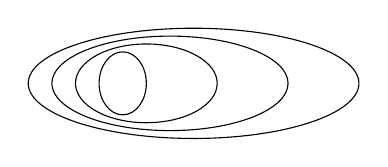
\begin{tikzpicture}
    %ellipses
    \draw (0,1) ellipse (0.3cm and 0.4cm);
    \draw (0.3,1) ellipse (0.9cm and 0.5cm);
    \draw (0.6,1) ellipse (1.5cm and 0.6cm);
    \draw (0.9,1) ellipse (2.1cm and 0.7cm);
    %math
    \draw (0,1) node[anchor=center] {$\N$};
    \draw (0.7,1) node[anchor=center] {$\Z$};
    \draw (1.6,1) node[anchor=center] {$\Q$};
    \draw (2.5,1) node[anchor=center] {$\R$};
\end{tikzpicture}\\
Later, we will see complex numbers.
In computer science, types matter a lot.

\subparagraph{Functions}
\begin{definition}[Functions]
    Assignment from a set to another.
\end{definition}
\begin{notation}[Function]
    $f: X \to Y$, $f(x)=blah$, $f: x \mapsto blah$.
\end{notation}
\begin{question}
    Which ones of these function are well-defined ?
    \begin{itemize}
        \item $f:k\in \{0,1,2,3,4\}\mapsto 24/k\in \N$
        \item $f:k\in \{1,2,3,4\}\mapsto 24/k\in \N$
        \item $f:k\in \{1,2,3,4,5\}\mapsto 24/k\in \N$
        \item $f:k\in \{1,2,3,4\}\mapsto k\in \{1,2\}$
        \item $f:k\in \{1,2,3,4\}\mapsto k\in \{1,2,3,4,5\}$
    \end{itemize}
\end{question}

\subparagraph{Quantifiers}
\begin{notation}[$\forall$]
    For all elements in set, e.g.: $\forall x \in \R, x^2 \geq 0$.
\end{notation}
\begin{notation}[$\exists$]
    There exists an element in set, e.g.: $\exists x \in \R \text{ s.t. } x^2 > 1$.
\end{notation}
\begin{notation}[$\exists !$]
    There exists a unique element in set, e.g.: $\exists ! x \in \R \text{ s.t. } x^2 \leq 0$.
\end{notation}
\begin{question}
    \begin{itemize}
        \item Express "all natural numbers are positive" with quantifiers
        \item Express $\forall x \geq 0, \ \sqrt{x} \geq 0$ in a sentence
    \end{itemize}
\end{question}
\begin{definition}[Subset / Inclusion]
    $X \subseteq Y$ if $\forall x \in X, x \in Y$
\end{definition}
\begin{definition}[Disjoint Sets]
    $X$ and $Y$ are disjoint if $\forall x \in X, x \not\in Y$ (or if $\forall y \in Y, y \not\in X$).
\end{definition}
\begin{definition}[Power Set]
    $\Pow{X} = \{ Y \mid Y \subseteq X \}$\\
    e.g.: $\Pow{\{1,2,3\}}=\{ \emptyset, \{1\},\{2\},\{3\}, \{1,2\},\{1,3\},\{2,3\}, \{1,2,3\} \}$
\end{definition}

\subparagraph{Scalars vs vectors}
1D vs 2D:\vspace{0.2cm}\\
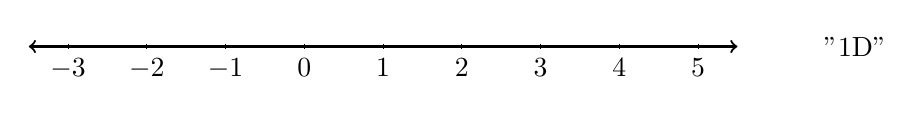
\begin{tikzpicture}
    \draw[thick,<->] (-3.5,0) -- (5.5,0);
    \foreach \x in {-3,-2,-1,0,1,2,3,4,5}
    \draw (\x cm,1pt) -- (\x cm,-1pt) node[anchor=north] {$\x$};
   \draw (7,0) node[anchor=center] {"1D"};
\end{tikzpicture}\\
\begin{tikzpicture}
    \draw[thick,<->] (-1.5,0) -- (3.5,0);
    \draw[thick,<->] (0,-1.5) -- (0,3.5);
    \foreach \x in {-1,1,2,3}
        \draw (\x cm,1pt) -- (\x cm,-1pt) node[anchor=north] {$\x$};
    \foreach \y in {-1,1,2,3}
        \draw (1pt,\y cm) -- (-1pt,\y cm) node[anchor=east] {$\y$};
    \draw (5,1) node[anchor=center] {"2D"};
\end{tikzpicture}\\
To "select" a point in 2D, we need 2 numbers, giving a coordinate.
In 3D, we would need 3 numbers, in 4D, 4 numbers, etc...
\begin{definition}[Cartesian Product]
    $X \times Y = \{ (x,y) \mid x \in X, y \in Y \}$\\
    e.g.: $\{a,b\} \times \{1,2,3\} = \{ (a,1),(a,2),(a,3), (b,1),(b,2),(b,3) \}$\\
    e.g.: $\R \times \R = \{ (x,y) \mid x,y \in \R \}$\\
    Extension: $X_1 \times \dots \times X_n = \prod_{k=1}^n X_k$
\end{definition}
Moving from one point to another gives a "translation".
Again, we need ad many numbers as there are dimensions.
Typically, we denote points horizontally, and vectors vertically.

\subsection{Axioms}
Here $ \star $ and $ \dagger $ will operations.
\begin{definition}[Associativity]
    $\star$ is associative if $\forall x,y,z, \ (x \star y) \star z = x \star (y \star z)$
\end{definition}
\begin{definition}[Commutativity]
    $\star$ is associative if $\forall x,y, \ (x \star y) = y \star x$
\end{definition}
\begin{definition}[Identity]
    $1_{\star}$ is identity for $\star$ if $\forall x, \ 1_{\star} \star x = x \star 1_{\star} = x$
\end{definition}
\begin{definition}[Annihilator]
    $0_{\star}$ is annihilator for $\star$ if $\forall x, \ 0_{\star} \star x = x \star 0_{\star} = 0_{\star}$
\end{definition}
\begin{definition}[Distributivity]
    $\star$ is distributive over $\dagger$ if $\forall x,y,z \ x \star (y \dagger z) = (x \star y) \dagger (x \star z)$
\end{definition}


 of $\land$ over $\lor$:  $x \land (y \lor z) = (x \land y) \lor (x \land z)$
\begin{question}
    \begin{itemize}\textit{(make a table)}
        \item Which of these are commutative: addition, subtraction, multiplication, division, power?
        \item Which of these are associative: addition, subtraction, multiplication, division, power?
        \item What is identity for: addition, subtraction, multiplication, division, power?
        \item What is annihilator for: addition, subtraction, multiplication, division, power?
    \end{itemize}
\end{question}
\begin{question}
    \begin{itemize}
        \item Think of an operation that is commutative, but not associative
        \item Think of an operation that is associative, but not commutative
    \end{itemize}
\end{question}


\subsection{Boolean algebra}
\textit{The reason we'll do some is because of it's application to programming, in particular to conditions ('if' blocks and 'while' loops).}
\subparagraph{Basic operators}
\begin{definition}[Conjunction]
    $x \land y = xy$
\end{definition}
\begin{definition}[Intersection]
    $X \cap Y = \{ z \mid (z \in X) \land (z \in Y) \}$
\end{definition}
\begin{remark}[Disjoint Sets and Intersection]
    Disjoint sets have empty intersection.
\end{remark}
\begin{definition}[Disjunction]
    $x \lor y = \min(x+y,1)$
\end{definition}
\begin{definition}[Union]
    $X \cup Y = \{ z \mid (z \in X) \lor (z \in Y) \}$
\end{definition}
\begin{definition}[Negation]
    $\lnot: 0,1 \mapsto 1,0$
\end{definition}
\begin{definition}[Set minus / Complement]
    $X \setminus Y = \{ x \in X \mid \lnot (x \in Y) \}$
\end{definition}
[Draw diagrams]
\begin{question}
    Selecting points outside a given region.
\end{question}
\subparagraph{Basic properties}
\begin{property}[Boolean algebra matching ordinary algebra]
    Same laws as ordinary algebra when one matches up $\lor$ with addition and $\land$ with multiplication.
    \begin{itemize}
        \item Associativity of $\lor$: $x \lor (y \lor z) = (x \lor y) \lor z$
        \item Associativity of $\land$: $x \land (y \land z) = (x \land y) \land z$
        \item Commutativity of $\lor$: $x \lor y  = y \lor x$
        \item Commutativity of $\land$: $x \land y  = y \land x$
        \item Distributivity of $\land$ over $\lor$:  $x \land (y \lor z) = (x \land y) \lor (x \land z)$
        \item $0$ is identity for $\lor$: $x \lor 0  = x$
        \item $1$ is identity for $\land$: $x \land 1  = x$
        \item $0$ is annihilator for $\land$: $x \land 0  = 0$
    \end{itemize}
\end{property}
\begin{property}[Boolean algebra specific properties]
    The following laws hold in Boolean algebra, but not in ordinary algebra: 
    \begin{itemize}
        \item Idempotence of $\lor$: $x \lor x = x$
        \item Idempotence of $\land$: $x \land x = x$
        \item Absorption of $\lor$ over $\land$: $x \lor (x \land y)  = x \land y$
        \item Absorption of $\land$ over $\lor$: $x \land (x \lor y)  = x \lor y$
        \item Distributivity of $\lor$ over $\land$:  $x \lor (y \land z) = (x \lor y) \land (x \lor z)$
        \item $1$ is annihilator for $\lor$: $x \lor 1 = 1$
    \end{itemize}
\end{property}
\begin{property}[De Morgan Laws]
    $\lnot (x \land y) = \lnot x \lor \lnot y$
    and
    $\lnot (x \lor y) = \lnot x \land \lnot y$
\end{property}
\begin{proof}
    Truth-tables; prove De Morgan, others as exercise (or just believe me)
\end{proof}

\subparagraph{Other operators}
\begin{definition}[Exclusive Or]
    $x \oplus y$
\end{definition}
\begin{definition}[Implication]
    $x \implies y$
\end{definition}
\begin{property}[Implication and Inclusion]
    If $\forall x \in X, P_1(x) \implies P_2(x)$, then $\{ x \in X \mid P_1(x) \} \subset \{ x \in X \mid P_2(x) \}$.
\end{property}
\begin{proof}
    Trivial.
\end{proof}
\begin{definition}[If and only if]
    $x \iff y$
\end{definition}
\begin{question}
    Express in terms of and, or, not:
    \begin{itemize}
        \item $\oplus$
        \item $\implies$
        \item $\impliedby$
        \item $\iff$
    \end{itemize}
    Write 1st and 2nd digit of addition of 3 binary numbers $a$, $b$, $c$.
\end{question}

\subparagraph{Negation of quantified propositions}
\begin{property}[Negation of $\forall$]
    $\mathrm{not}(\forall x\in X, P(x)) = \exists x\in X, \mathrm{not}(P(x))$
\end{property}
\begin{property}[Negation of $\exists$]
    $\mathrm{not}(\exists x\in X, P(x)) = \forall x\in X, \mathrm{not}(P(x))$
\end{property}
\begin{notation}[Quantifiers and the empty set]
    $\forall x \in \emptyset, \ \dots$ is true ;
    $\exists x \in \emptyset, \ \dots$ is false
\end{notation}
\begin{question} Negate the following
    \begin{itemize}
        \item $\forall x \in \R, \ \exists n \in \N \text{ s.t. } n > x$
        \item ($x_n \to x$): $\forall \epsilon>0, \exists N \in \N \text{ s.t. } \forall n>N, \abs{x_n-x}<\epsilon$
    \end{itemize}
\end{question}



\subsection{Objects \& Notations}
- $\N$, $\Z$, $\Q$, $\R$
- scalars vs vectors
\subsection{Proofs}
Example of proofs and non-proofs
- direct
- splitting cases
- induction
- contradiction
\subsection{Geometry}
- equations of lines/planes, etc... => vectors / scalar \& equation manipulations
\subsection{Sets}
- min/max \& sup/inf => start using for all / there exists
\subsection{Integers}
- prime numbers (infinite nb by Euclide)
- unique factorization 
- finding primes between 1 and 100 => time complexity of algo?